\documentclass[tikz,border=1mm,10pt]{standalone}
%\usepackage[dvipsnames]{xcolor}
\usepackage{pgfplots}
\pgfplotsset{compat=1.5.1}
\usetikzlibrary{arrows}
\begin{document}
	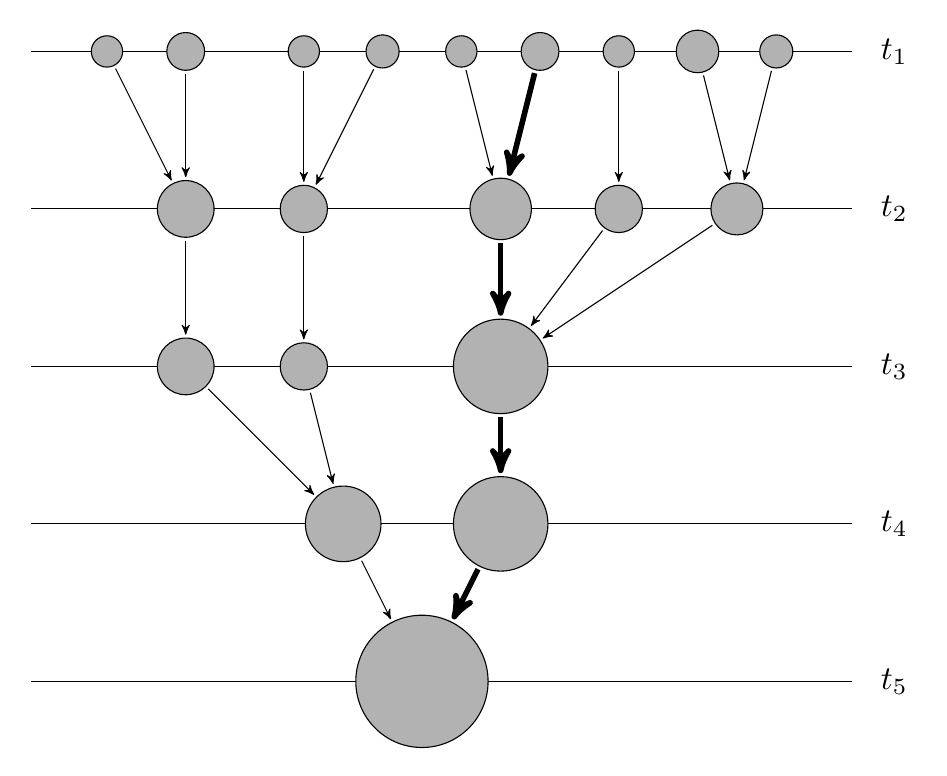
\begin{tikzpicture}[xscale=1,yscale=1,samples=400, transform shape,every node/.style={scale=1.2}, shorten <=1pt, shorten >=1pt]


        %===========================
        % Timelines
        %===========================
        
        \draw (5,0) -- (15.5, 0);
        \draw (5,2) -- (15.5, 2);
        \draw (5,4) -- (15.5, 4);
        \draw (5,6) -- (15.5, 6);
        \draw (5,8) -- (15.5, 8);
        \node at (16,8) {$t_1$};
        \node at (16,6) {$t_2$};
        \node at (16,4) {$t_3$};
        \node at (16,2) {$t_4$};
        \node at (16,0) {$t_5$};
        
        
        
        %===========================
        % Haloes
        %===========================        
        \draw node (A) at (10,0) [fill=gray!60,circle,minimum size=1.4cm, draw]{};

        % Left Side
        \draw node (B1) at (9,2) [fill=gray!60,circle,minimum size=0.8cm, draw]{}; 
        \draw[-stealth'] (B1) to (A);      

        \draw node (C1) at (7,4) [fill=gray!60,circle,minimum size=0.6cm, draw]{}; 
        \draw[-stealth'] (C1) to (B1);      
        \draw node (C2) at (8.5,4) [fill=gray!60,circle,minimum size=0.5cm, draw]{};
        \draw[-stealth'] (C2) to (B1);
        
        \draw node (D1) at (7,6) [fill=gray!60,circle,minimum size=0.6cm, draw]{}; 
        \draw[-stealth'] (D1) to (C1);      
        \draw node (D2) at (8.5,6) [fill=gray!60,circle,minimum size=0.5cm, draw]{};
        \draw[-stealth'] (D2) to (C2);      
        
        \draw node (E1) at (6,8) [fill=gray!60,circle,minimum size=0.25cm, draw]{};
        \draw[-stealth'] (E1) to (D1);
        \draw node (E2) at (7,8) [fill=gray!60,circle,minimum size=0.4cm, draw]{}; 
        \draw[-stealth'] (E2) to (D1);      
        \draw node (E3) at (8.5,8) [fill=gray!60,circle,minimum size=0.2cm, draw]{};
        \draw[-stealth'] (E3) to (D2);
        \draw node (E4) at (9.5,8) [fill=gray!60,circle,minimum size=0.35cm, draw]{}; 
        \draw[-stealth'] (E4) to (D2);  
        
        
        % Right Side    
        \draw node (B2) at (11,2) [fill=gray!60,circle,minimum size=1cm, draw]{};
        \draw[-stealth', line width=2pt] (B2) to (A);
        
        \draw node (C3) at (11,4) [fill=gray!60,circle,minimum size=1cm, draw]{}; 
        \draw[-stealth', line width=2pt] (C3) to (B2);      
        
        \draw node (D3) at (11,6) [fill=gray!60,circle,minimum size=0.65cm, draw]{}; 
        \draw[-stealth', line width=2pt] (D3) to (C3);      
        \draw node (D4) at (12.5,6) [fill=gray!60,circle,minimum size=0.5cm, draw]{};
        \draw[-stealth'] (D4) to (C3);      
        \draw node (D5) at (14,6) [fill=gray!60,circle,minimum size=0.55cm, draw]{};
        \draw[-stealth'] (D5) to (C3);

        
        \draw node (E5) at (10.5,8) [fill=gray!60,circle,minimum size=0.2cm, draw]{};
        \draw[-stealth'] (E5) to (D3);
        \draw node (E6) at (11.5,8) [fill=gray!60,circle,minimum size=0.4cm, draw]{}; 
        \draw[-stealth', line width=2pt] (E6) to (D3);      
        \draw node (E7) at (12.5,8) [fill=gray!60,circle,minimum size=0.2cm, draw]{};
        \draw[-stealth'] (E7) to (D4);
        \draw node (E8) at (13.5,8) [fill=gray!60,circle,minimum size=0.45cm, draw]{}; 
        \draw[-stealth'] (E8) to (D5);
        \draw node (E9) at (14.5,8) [fill=gray!60,circle,minimum size=0.35cm, draw]{}; 
        \draw[-stealth'] (E9) to (D5);              
	\end{tikzpicture}
\end{document}